\Aufgabe[20]{Wdh: Von der Klasse zur Tabelle}{
    \begin{itemize}
        \item Zeichnet zu zweit eine Tabelle, in der man alle Objekte der Klasse Person sammeln kann.
        \item Tragt eure beiden Objekte (vom Objektkarten-Memory) in die Tabelle ein.
        \item Ordnet die folgenden Begriffe den Teilen der Tabelle zu.
            \\Achtung: Nicht alle Begriffe passen und manches hat mehrere Begriffe!
            \\
        \emphColB{Datensatz~~~ Tabelle~~~ Zelle~~~ Klasse~~~ Objekt~~~ Parameter~~~ Attribut~~~ Spalte~~~ Feld~~~ Methode~~~ Board~~~ Zeile~~~ Datentyp~~~ Attributwert}
    \end{itemize}
    \LoesungKaro{
        Lösung:
        
        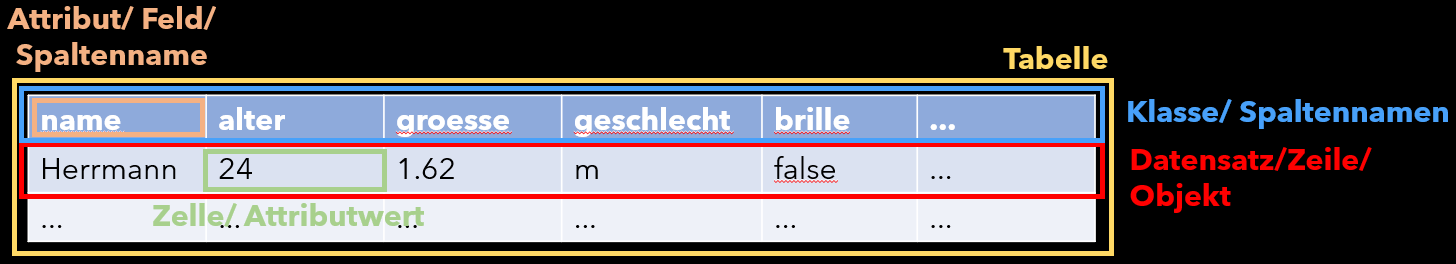
\includegraphics[width=\textwidth]{_Aufgaben/img/A01_Lsg.png}

        Nicht verwendete Begriffe: Parameter, Methode, Board, Datentyp

        \footnotesize
        Feld: Wird oft synonym zu Attribut verwendet, v.a. in Programmen wie LibreOffice Base oder MS Access.
    }{17}
}
